\documentclass[11pt]{article}

% PACKAGES
\usepackage{amsmath}
\usepackage{amssymb}
\usepackage{graphicx}
\usepackage[margin=1in]{geometry}
\usepackage{hyperref}
\usepackage{tikz}
\usetikzlibrary{decorations.markings}
\usetikzlibrary{arrows.meta}

% DOCUMENT INFO
\title{Concise Notes and Problems on Electromagnetic Induction}
\author{}
\date{\today}

\begin{document}

\maketitle
\tableofcontents
\newpage

\section{Notes on Electromagnetic Induction (EMI)}

\subsection{What is Electromagnetic Induction? \_a}
Electromagnetic induction is the process of generating an electromotive force (EMF), which is essentially a voltage, in a conductor by changing the magnetic field around it. A changing magnetic field creates an electric field. This discovery by Michael Faraday is the principle behind electric generators, transformers, and induction cooktops.

\subsection{Magnetic Flux ($\Phi_B$)}
Magnetic flux is a measure of the total magnetic field lines passing through a given area.

\begin{itemize}
    \item \textbf{Equation:} For a uniform magnetic field $\vec{B}$ passing through a flat area $\vec{A}$, the flux is:
    $$ \Phi_B = \vec{B} \cdot \vec{A} = BA\cos\theta $$
    where $\theta$ is the angle between the magnetic field $\vec{B}$ and the normal to the area, $\vec{A}$.
    
    \begin{center}
    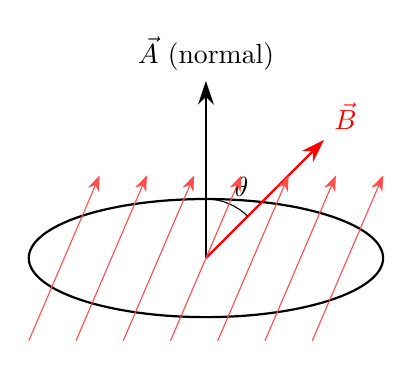
\begin{tikzpicture}[scale=1.5]
        % Draw the loop
        \draw[thick] (0,0) ellipse (1.5cm and 0.5cm);
        % Draw the normal vector
        \draw[-{Stealth[length=3mm, width=2mm]}, thick] (0,0) -- (0,1.5) node[above] {$\vec{A}$ (normal)};
        % Draw the B-field vector
        \draw[-{Stealth[length=3mm, width=2mm]}, thick, red] (0,0) -- (1,1) node[above right] {$\vec{B}$};
        % Draw the angle
        \draw (0,0.5) arc (90:45:0.5cm);
        \node at (0.3,0.6) {$\theta$};
        % Draw some B-field lines passing through
        \foreach \x in {-1.2,-0.8,-0.4,0,0.4,0.8,1.2}{
            \draw[-{Stealth[length=2mm]}, red!70] (\x-0.3, -0.7) -- (\x+0.3, 0.7);
        }
    \end{tikzpicture}
    \end{center}
    
    \item \textbf{Unit:} The SI unit for magnetic flux is the Weber (Wb), where $1~\text{Wb} = 1~\text{T} \cdot \text{m}^2$.
    
    \item \textbf{Key Idea:} You can change the flux by changing the \textbf{magnetic field strength (B)}, the \textbf{area of the loop (A)}, or the \textbf{orientation of the loop ($\theta$)}.
\end{itemize}

\subsection{Faraday's Law of Induction}
This law quantifies the induced EMF. It states that the magnitude of the induced EMF ($\mathcal{E}$) in a loop is directly proportional to the rate of change of magnetic flux through the loop.

\begin{itemize}
    \item \textbf{Equation:}
    $$ \mathcal{E} = -N \frac{d\Phi_B}{dt} $$
    \begin{itemize}
        \item $\mathcal{E}$ is the induced EMF (in Volts).
        \item $N$ is the number of turns in the coil.
        \item $\frac{d\Phi_B}{dt}$ is the rate of change of magnetic flux (in Wb/s).
    \end{itemize}
\end{itemize}

\subsection{Lenz's Law (The ``-'' Sign)}
The negative sign in Faraday's Law is crucial and is represented by Lenz's Law. It tells us the \textbf{direction} of the induced current.
\begin{itemize}
    \item \textbf{Principle:} The induced current will flow in a direction that creates its own magnetic field to \textbf{oppose the change in magnetic flux} that produced it.
    \item \textbf{Analogy:} Think of it as "magnetic inertia." Nature resists changes in magnetic flux.
    \begin{itemize}
        \item If flux is \textbf{increasing}, the induced field will point in the opposite direction to the original field.
        \item If flux is \textbf{decreasing}, the induced field will point in the same direction as the original field to try and prop it up.
    \end{itemize}
\end{itemize}

\begin{center}
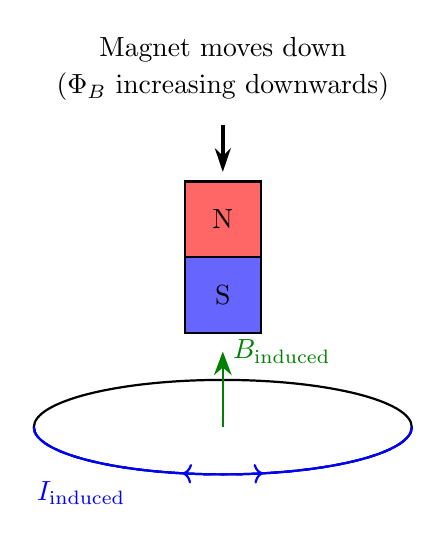
\begin{tikzpicture}[scale=1.2]
    % --- Corrected Lenz's Law Diagram ---
    % Text description
    \node at (0, 4) {Magnet moves down};
    \node at (0, 3.6) {($\Phi_B$ increasing downwards)};
    
    % Velocity vector
    \draw[-{Stealth[length=3mm, width=2mm]}, ultra thick] (0, 3.2) -- (0, 2.7);

    % Bar magnet
    \draw[thick, fill=blue!60] (-0.4, 1.8) rectangle (0.4, 1);
    \node at (0, 1.4) {S};
    \draw[thick, fill=red!60] (-0.4, 2.6) rectangle (0.4, 1.8);
    \node at (0, 2.2) {N};

    % Coil
    \draw[thick] (0,0) ellipse (2cm and 0.5cm);
    
    % Induced B-field (upwards, opposing the change)
    \draw[-{Stealth[length=3mm]}, thick, green!50!black] (0, 0) -- (0, 0.8) node[right] {$B_{\text{induced}}$};
    
    % Induced current (counter-clockwise)
    \begin{scope}[decoration={
        markings,
        mark=at position 0.6 with {\arrow{>}}}
        ]
        % Front part of the coil's current arrow
        \draw[postaction={decorate}, thick, blue] (2,0) arc (0:-180:2cm and 0.5cm);
        % Back part of the coil's current arrow (dashed)
        \draw[postaction={decorate}, thick, blue, dashed] (-2,0) arc (180:360:2cm and 0.5cm);
    \end{scope}
    \node[blue] at (-1.5, -0.7) {$I_{\text{induced}}$};
\end{tikzpicture}
\end{center}

\subsection{Motional EMF}
This is the EMF induced in a conductor moving through a magnetic field.
\begin{itemize}
    \item \textbf{Scenario:} A conductor of length $L$ moves at a constant velocity $\vec{v}$ perpendicular to a uniform magnetic field $\vec{B}$.
    \item \textbf{Equation:}
    $$ \mathcal{E} = BLv $$
\end{itemize}
\begin{center}
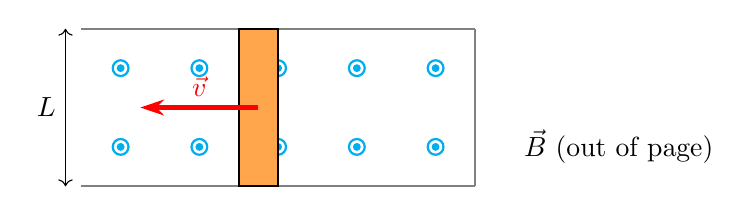
\begin{tikzpicture}
    % Rails
    \draw[thick, gray] (0,2) -- (5,2);
    \draw[thick, gray] (0,0) -- (5,0);
    \draw[thick, gray] (5,0) -- (5,2);
    % B-field
    \foreach \x in {0.5,1.5,...,4.5}
        \foreach \y in {0.5,1.5}
            \draw[cyan, thick] (\x,\y) circle (0.1cm);
    \foreach \x in {0.5,1.5,...,4.5}
        \foreach \y in {0.5,1.5}
            \fill[cyan] (\x,\y) circle (0.05cm);
    \node at (5.5,0.5) [right] {$\vec{B}$ (out of page)};
    % Rod
    \draw[thick, fill=orange!70] (2,0) rectangle (2.5,2);
    % Velocity vector
    \draw[-{Stealth[length=3mm, width=2mm]}, ultra thick, red] (2.25,1) -- (0.75,1) node[midway, above] {$\vec{v}$};
    % Length L
    \draw[<->] (-0.2,0) -- (-0.2,2) node[midway, left] {$L$};
\end{tikzpicture}
\end{center}
\subsection{Energy Conservation \_b}
The energy for the induced current comes from the work done to move the conductor.
\begin{itemize}
    \item The induced current $I$ creates a \textbf{magnetic drag force}, $F_m = ILB$, which opposes the motion.
    \item To maintain constant velocity, an \textbf{external force} $F_{ext} = ILB$ must be applied.
    \item The \textbf{mechanical power} supplied is $P_{\text{mech}} = F_{\text{ext}}v = (ILB)v$.
    \item The \textbf{electrical power} dissipated as heat is $P_{\text{elec}} = I^2R$.
    \item By conservation of energy: $P_{\text{mech}} = P_{\text{elec}}$.
\end{itemize}


\newpage
\section{Problem Solutions}

\subsection{Problem 1 (from EMI3.pdf)}
\textbf{Given:} $L = 10 \text{ cm} = 0.10 \text{ m}$, $v = 5.0 \text{ m/s}$, $B = 1.2 \text{ T}$, $R_{\text{rod}} = 0.40 \, \Omega$.

\begin{enumerate}
    \item[(a)] \textbf{Magnitude of the induced EMF}
    $$ \mathcal{E} = BLv = (1.2 \text{ T})(0.10 \text{ m})(5.0 \text{ m/s}) = \mathbf{0.60 \, V} $$

    \item[(b)] \textbf{Direction of the induced EMF}
    Using the Lorentz force on positive charge carriers, $\vec{F} = q(\vec{v} \times \vec{B})$. The velocity $\vec{v}$ is to the left, and the magnetic field $\vec{B}$ is out of the page. The resulting force $\vec{F}$ is downwards. Therefore, the direction of the EMF is \textbf{down}.

    \item[(c)] \textbf{Magnitude of the current}
    $$ I = \frac{\mathcal{E}}{R} = \frac{0.60 \text{ V}}{0.40 \, \Omega} = \mathbf{1.5 \, A} $$
    
    \item[(d)] \textbf{Direction of the current}
    The EMF acts like a battery with the positive terminal at the bottom of the rod. Current flows from positive to negative through the external circuit, resulting in a \textbf{counter-clockwise} loop.

    \item[(e)] \textbf{Rate of thermal energy generation}
    $$ P_{\text{thermal}} = I^2R = (1.5 \text{ A})^2 (0.40 \, \Omega) = \mathbf{0.90 \, W} $$
    
    \item[(f)] \textbf{External force needed}
    The external force must balance the magnetic drag force, $F_m = ILB$.
    $$ F_{\text{ext}} = ILB = (1.5 \text{ A})(0.10 \text{ m})(1.2 \text{ T}) = \mathbf{0.18 \, N} $$
    The force must be applied in the direction of motion, to the \textbf{left}.
    
    \item[(g)] \textbf{Rate at which the external force does work}
    $$ P_{\text{force}} = F_{\text{ext}}v = (0.18 \text{ N})(5.0 \text{ m/s}) = \mathbf{0.90 \, W} $$
    This matches the thermal energy rate, as expected from energy conservation.
\end{enumerate}
\hrule

\subsection{Problem 2 (from EMI1.pdf)}
This problem involves a conductor moving on V-shaped rails, where the length of the conductor in the circuit changes as it moves.

\begin{center}
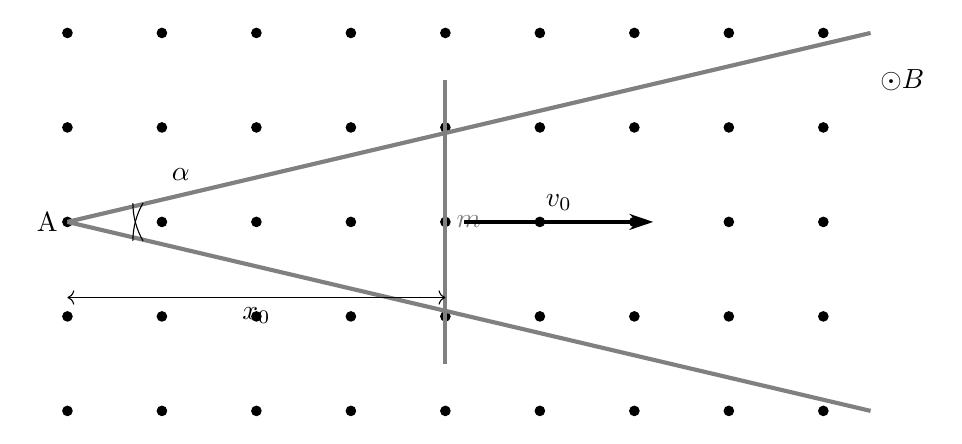
\begin{tikzpicture}[scale=1.2]
    % B-field (dots)
    \foreach \x in {0,1,...,8}
        \foreach \y in {0,1,...,4}
            \filldraw (\x,\y) circle (0.05cm);
    \node at (8.5, 3.5) [right] {$\odot B$};

    % V-shaped wire
    \draw[thick, gray, line width=1.5pt] (0,2) -- (8.5,4);
    \draw[thick, gray, line width=1.5pt] (0,2) -- (8.5,0);
    \node at (0,2) [left] {A};

    % Angle alpha
    \draw (0.8, 2.2) arc (150:180:0.8);
    \draw (0.8, 1.8) arc (210:180:0.8);
    \node at (1.2, 2.5) {$\alpha$};
    
    % Rod
    \draw[thick, gray, fill=white, line width=1.5pt] (4,0.5) -- (4,3.5) node[midway, right] {$m$};
    
    % Initial position and velocity
    \draw[<->] (0,1.2) -- (4,1.2) node[midway, below] {$x_0$};
    \draw[-{Stealth[length=3mm, width=2mm]}, ultra thick] (4.2, 2) -- (6.2, 2) node[midway, above] {$v_0$};
\end{tikzpicture}
\end{center}

\begin{enumerate}
    \item \textbf{Define variables at position $x$:}
    The half-angle of the V-shape is $\frac{\alpha}{2}$.
    \begin{itemize}
        \item The length of the rod in the circuit is $L(x) = 2x \tan(\frac{\alpha}{2})$.
        \item The resistance of the rod is $R_{\text{rod}}(x) = R \cdot L(x) = 2Rx \tan(\frac{\alpha}{2})$.
    \end{itemize}

    \item \textbf{Calculate Induced EMF and Current:}
    \begin{itemize}
        \item Motional EMF: $\mathcal{E} = B L(x) v = B (2x \tan(\frac{\alpha}{2})) v$.
        \item Induced Current: $I = \frac{\mathcal{E}}{R_{\text{rod}}(x)} = \frac{B (2x \tan(\frac{\alpha}{2})) v}{2Rx \tan(\frac{\alpha}{2})} = \frac{Bv}{R}$.
        \item The current $I$ is independent of position $x$.
    \end{itemize}
    
    \item \textbf{Set up the Equation of Motion:}
    The magnetic drag force $F_m$ opposes the motion.
    $$ F_m = I L(x) B = \left(\frac{Bv}{R}\right) \left(2x \tan\left(\frac{\alpha}{2}\right)\right) B = \frac{2B^2v \tan(\frac{\alpha}{2})}{R} x $$
    Using Newton's Second Law ($F_{\text{net}} = ma$):
    $$ m \frac{dv}{dt} = -F_m = -\frac{2B^2 \tan(\frac{\alpha}{2})}{R} x v $$
    
    \item \textbf{Solve the Differential Equation:}
    Use the chain rule: $a = \frac{dv}{dt} = \frac{dv}{dx}\frac{dx}{dt} = v\frac{dv}{dx}$.
    $$ m v\frac{dv}{dx} = -\frac{2B^2 \tan(\frac{\alpha}{2})}{R} x v $$
    Cancel $v$ from both sides and separate variables:
    $$ m \, dv = -\frac{2B^2 \tan(\frac{\alpha}{2})}{R} x \, dx $$
    Integrate from initial state ($v_0, x_0$) to final state ($0, x$):
    $$ \int_{v_0}^{0} m \, dv = \int_{x_0}^{x} -\frac{2B^2 \tan(\frac{\alpha}{2})}{R} x \, dx $$
    $$ m[v]_{v_0}^{0} = -\frac{2B^2 \tan(\frac{\alpha}{2})}{R} \left[\frac{x^2}{2}\right]_{x_0}^{x} $$
    $$ m(0 - v_0) = -\frac{B^2 \tan(\frac{\alpha}{2})}{R} (x^2 - x_0^2) $$
    $$ mv_0 = \frac{B^2 \tan(\frac{\alpha}{2})}{R} (x^2 - x_0^2) $$
    Rearranging to solve for the final position $x$:
    $$ x^2 - x_0^2 = \frac{mv_0 R}{B^2 \tan(\frac{\alpha}{2})} $$
    $$ \mathbf{x = \sqrt{x_0^2 + \frac{mv_0 R}{B^2 \tan(\frac{\alpha}{2})}}} $$
    This matches the required expression.
\end{enumerate}
\hrule

\subsection{Problem 3 (from EMI2.pdf)}
\textbf{Given:} $m = 20 \text{ g} = 0.020 \text{ kg}$, $R = 1.2 \, \Omega$, $L = 50 \text{ cm} = 0.50 \text{ m}$, $B = 40 \text{ mT} = 0.040 \text{ T}$.

\begin{center}
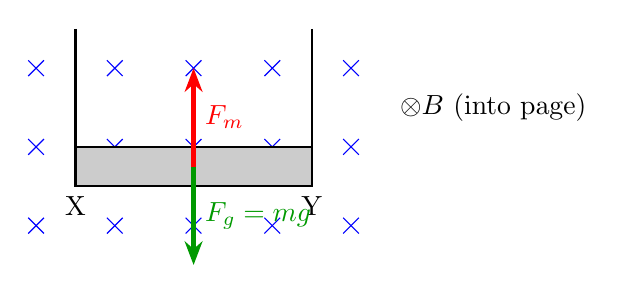
\begin{tikzpicture}
    % B-field (crosses)
    \foreach \x in {0.5,1.5,...,4.5}
        \foreach \y in {-0.5,0.5,1.5}
            \draw[blue] (\x-0.1, \y-0.1) -- (\x+0.1, \y+0.1);
    \foreach \x in {0.5,1.5,...,4.5}
        \foreach \y in {-0.5,0.5,1.5}
            \draw[blue] (\x-0.1, \y+0.1) -- (\x+0.1, \y-0.1);
    \node at (5, 1) [right] {$\otimes B$ (into page)};

    % Suspended Wire
    \draw[thick] (1,2) -- (1,0.5);
    \draw[thick] (4,2) -- (4,0.5);
    \draw[thick, fill=gray!40] (1,0.5) rectangle (4,0);
    \node at (1, -0.25) {X};
    \node at (4, -0.25) {Y};
    
    % Forces
    \draw[-{Stealth[length=3mm]}, ultra thick, red] (2.5,0.25) -- (2.5,1.5) node[midway, right] {$F_m$};
    \draw[-{Stealth[length=3mm]}, ultra thick, green!60!black] (2.5,0.25) -- (2.5,-1) node[midway, right] {$F_g = mg$};
\end{tikzpicture}
\end{center}

\begin{enumerate}
    \item \textbf{Condition for Zero Tension:}
    For zero tension, the upward magnetic force ($F_m$) must balance the downward gravitational force ($F_g$).
    $$ F_m = F_g $$
    
    \item \textbf{Calculate the Required Current:}
    $$ F_g = mg = (0.020 \text{ kg})(9.8 \text{ m/s}^2) = 0.196 \text{ N} $$
    $$ F_m = ILB \implies I = \frac{mg}{LB} = \frac{0.196 \text{ N}}{(0.50 \text{ m})(0.040 \text{ T})} = \mathbf{9.8 \, A} $$

    \item \textbf{Determine the Potential Difference:}
    Using Ohm's Law:
    $$ V = IR = (9.8 \text{ A})(1.2 \, \Omega) = \mathbf{11.76 \, V} \approx 12 \, \text{V} $$
    
    \item \textbf{Determine the Direction:}
    To get an upward force ($\vec{F}$) with a magnetic field ($\vec{B}$) into the page, the Right-Hand Rule ($\vec{F} = I(\vec{L} \times \vec{B})$) dictates that the current ($I$) must flow from left to right. Therefore, current flows from \textbf{X to Y}, meaning \textbf{X must be at a higher potential than Y}.
\end{enumerate}
\hrule

\subsection{Problem 4 (from EMI4.pdf)}
A conducting rod of length $l$ and resistance $R$ rotates at a constant angular velocity $\omega$ in a uniform magnetic field $B$. It is connected to an external resistor $R_0$.

\begin{center}
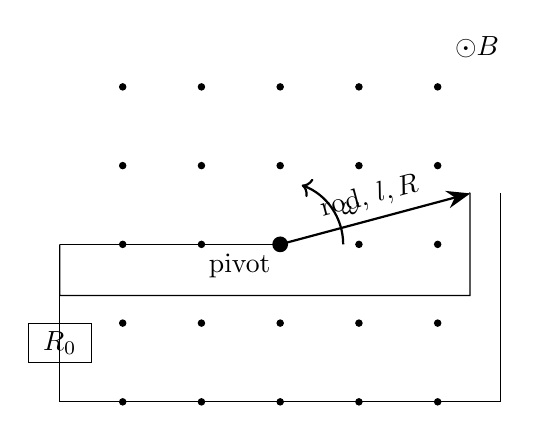
\begin{tikzpicture}
    % B-field (dots)
    \foreach \x in {-2,-1,...,2}
        \foreach \y in {-2,-1,...,2}
            \filldraw (\x,\y) circle (0.04cm);
    \node at (2.5, 2.5) {$\odot B$};

    % Rotating Rod
    \draw[thick, -{Stealth[length=3mm]}] (0,0) -- (15:2.5cm) node[midway, above, sloped] {rod, $l, R$};
    \fill (0,0) circle (0.1cm) node[below left] {pivot};
    \draw[->, thick] (0.8,0) arc (0:70:0.8cm) node[midway, right] {$\omega$};

    % External Circuit
    \draw (0,0) -- (-2.8, 0);
    \draw (15:2.5cm) -- (2.41, 0.65) -- (2.41, -0.65) -- (-2.8, -0.65) -- (-2.8, 0);
    % Resistor R0
    \draw (-2.8, -0.65) -- (-2.8, -1);
    \draw (-3.2, -1) rectangle (-2.4, -1.5);
    \node at (-2.8, -1.25) {$R_0$};
    \draw (-2.8, -1.5) -- (-2.8, -2);
    \draw (-2.8, -2) -- (-2.8, -0.65) [xshift=5.6cm];
    \draw (-2.8, -2) -- (2.8, -2) -- (2.8, 0.65);
\end{tikzpicture}
\end{center}

\begin{enumerate}
    \item[(a)] \textbf{What is the emf induced in the rod?}
    A small segment $dr$ at distance $r$ from the pivot has velocity $v = \omega r$. The EMF across it is $d\mathcal{E} = Bv \, dr = B(\omega r) \, dr$.
    To find the total EMF, we integrate from $r=0$ to $r=l$:
    $$ \mathcal{E} = \int_{0}^{l} B\omega r \, dr = B\omega \left[ \frac{r^2}{2} \right]_{0}^{l} $$
    $$ \mathcal{E} = \frac{1}{2} B\omega l^2 $$
    
    \item[(b)] \textbf{Determine the electric power developed in the resistor.}
    Total resistance of the series circuit is $R_{\text{total}} = R + R_0$.
    The current is $I = \frac{\mathcal{E}}{R_{\text{total}}} = \frac{B\omega l^2}{2(R + R_0)}$.
    The power in the external resistor $R_0$ is $P_{R_0} = I^2 R_0$:
    $$ P_{R_0} = \left( \frac{B\omega l^2}{2(R + R_0)} \right)^2 R_0 = \frac{B^2\omega^2 l^4 R_0}{4(R + R_0)^2} $$
    
    \item[(c)] \textbf{Describe, with evidence, the origin of the electric power.}
    \textbf{Origin:} The electric power originates from the \textbf{mechanical work} done by an external torque to keep the rod rotating at a constant angular velocity against the magnetic drag torque.

    \textbf{Evidence (Energy Conservation):}
    \begin{itemize}
        \item The current $I$ creates a magnetic force $dF_m = I B dr$ on each segment $dr$.
        \item This force creates a drag torque $d\tau_m = r \, dF_m = rIB \, dr$.
        \item The total magnetic drag torque is:
        $$ \tau_m = \int_{0}^{l} rIB \, dr = IB \left[ \frac{r^2}{2} \right]_{0}^{l} = \frac{1}{2} IBl^2 $$
        \item To maintain constant $\omega$, an external torque $\tau_{\text{ext}} = \tau_m$ must be applied.
        \item The mechanical power supplied is $P_{\text{mech}} = \tau_{\text{ext}} \omega = (\frac{1}{2} IBl^2) \omega$.
        \item The total electrical power dissipated in the circuit is $P_{\text{elec}} = I^2 R_{\text{total}} = I^2(R+R_0)$.
        \item Since $I = \frac{\mathcal{E}}{R+R_0}$ and $\mathcal{E} = \frac{1}{2}B\omega l^2$, we can write $I(R+R_0) = \mathcal{E}$.
        \item Let's check if $P_{\text{mech}} = P_{\text{elec}}$:
        $$ P_{\text{mech}} = \omega \left( \frac{1}{2}Bl^2 \right) I = \mathcal{E}I $$
        $$ P_{\text{elec}} = I^2(R+R_0) = I \cdot (I(R+R_0)) = I\mathcal{E} $$
        Since $P_{\text{mech}} = \mathcal{E}I$ and $P_{\text{elec}} = \mathcal{E}I$, the mechanical power supplied by the external torque is equal to the total electrical power dissipated in the circuit. This confirms the origin of the power.
    \end{itemize}
\end{enumerate}

\end{document}